%%Agregar +-
\section{Análisis y discusión de los resultados}

Con el objetivo de observar la relación entre el valor F1 alcanzado y el número de $n$ documentos aumentados 
%para el conjunto de depresión,
se presentan la figuras \ref{fig:aumento_n_depresion} y \ref{fig:aumento_n_anorexia}. En las gráficas se comparan los métodos: sin aumento de datos, sin restricción, restricción $\chi^2$ , relación equivalente y relación contraria. De acuerdo a la tabla \ref{table:resultados} estos fueron los métodos que superaron o igualaron a los métodos de referencia. El balance en el conjunto de depresión se alcanza con $n=4$. Las gráficas 
%de la figura\ref{fig:aumento_n_depresion}
se presentan en una escala de 0 a 100\% para el valor $F1$, el eje $x$ refleja el número de documentos aumentados durante el entrenamiento y el eje $y$ la ganancia en $F1$ en comparación con la línea base que es no realizar aumento de datos. 

En la figura \ref{fig:aumento_n_depresion} (a), el aumento para la red bidireccional, el mejor resultado con una ganancia de 6 puntos se obtiene con $n=7$ con el método \textit{Restricción Chi2}. Se puede observar que una vez alcanzado el balance de los datos empieza a mejorar la ganancia en F1 y después de $n=7$ empieza a decrecer. Sin embargo, el método de relaciones equivalentes y contrarias se mantienen en orden creciente, esto puede indicar que estos métodos son más robustos frente a un gran número de documentos. Por otro lado el método \textit{Sin restricción} comienza a decaer antes que el de restricción, esto indica que preferible mantener términos discriminantes o términos más relacionados a la clase a aumentar.

En la figura \ref{fig:aumento_n_depresion} (b), aumento de datos para la red CNN, el mejor valor encontrado con una ganancia de 5.2 puntos fue con $n=9$ con el método \textit{Restricción $\chi^2$}. A diferencia de la red recurrente las ganancias en F1 se encuentran en un rango entre 2 y 5 puntos, los métodos con menor ganancia fueron; el sin restricción y el basado relaciones contrarias, es importante mencionar el umbral de decisión final (decidir a que clase pertenece) se fijó en 0.4 como se sugiere en \cite{trotzek2018word}. 

En la figura \ref{fig:aumento_n_depresion} (c), aumento de datos para SVM, se presenta una tendencia creciente en relación al parámetro $n$, el mejor valor obtenido es una ganancia de 38 puntos mediante el método \textit{Restricción $\chi^2$}. En este caso la ganancia se debe más a la afectación de los pesos \textit{tf-idf} que al aumento de datos, aún así el método basado en restricción $\chi^2$ ofrece una mejora desde el primer documento en comparación con los otros métodos.

La figura \ref{fig:aumento_n_anorexia} (a) presenta el aumento de datos para el conjunto de anorexia y el modelo Bi-LSTM. La ganancia máxima se alcanza con el método basado en relaciones contrarias con 4.18 puntos. La ganancia comienza a aumentar a partir punto de balance con $n=3$. 

La figura \ref{fig:aumento_n_anorexia} (b) presenta el aumento de datos para el conjunto de anorexia en el modelo CNN. La ganancia obtenida se encuentra entre 0 y 3 puntos. En este caso los métodos tienen un comportamiento muy similar.

La figura \ref{fig:aumento_n_anorexia} (c) presenta el aumento de datos para el conjunto de anorexia en el modelo lineal SVM. En esta figura se puede observar que el método basado en relaciones contrarias obtiene la mejor ganancia con 13 puntos.
\newpage

\begin{figure}[hbt!]
    \begin{center}
    \begin{subfigure}[b]{0.6\textwidth}
        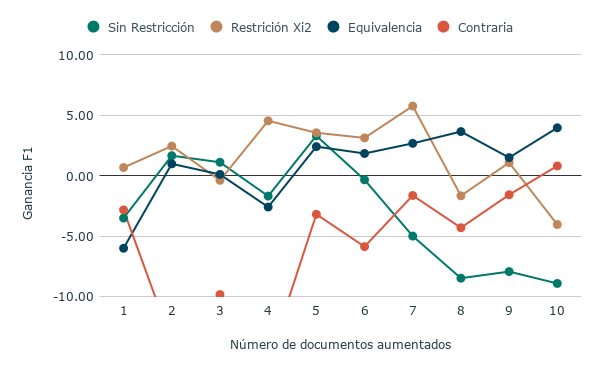
\includegraphics[width=\textwidth]{sections/figures/Bi-LSTM-dep.png}
        \caption{Bi-LSTM}
    \end{subfigure}
    \hfill
    
    \begin{subfigure}[!h]{0.6\textwidth}
        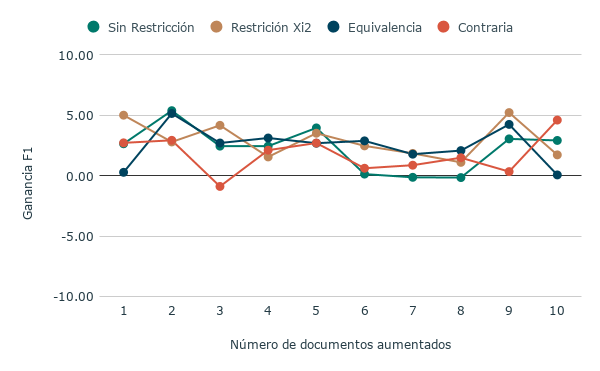
\includegraphics[width=\textwidth]{sections/figures/CNN_dep.png}
        \caption{CNN}
    \end{subfigure}
  
    \begin{subfigure}[b]{0.6\textwidth}
        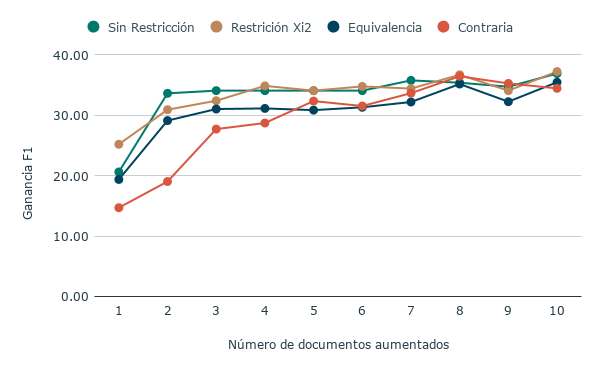
\includegraphics[width=\textwidth]{sections/figures/SVM_dep.png}
        \caption{SVM}
    \end{subfigure}
    \end{center}
   
    \caption{Relación entre el número de documentos aumentados y la ganancia en F1 para el conjunto \textit{Depresión}.}
    \label{fig:aumento_n_depresion}
\end{figure}


\newpage
\begin{figure}[hbt!]
    \centering
    \begin{subfigure}[b]{0.6\textwidth}
        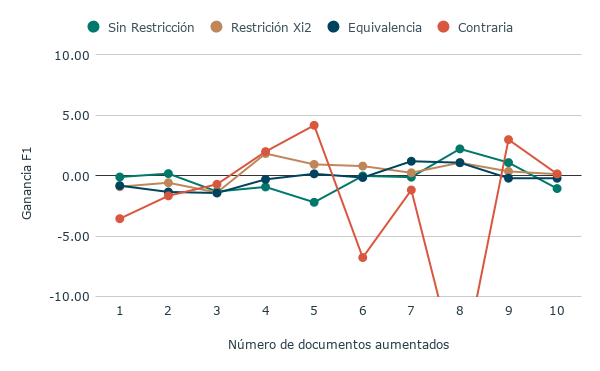
\includegraphics[width=\textwidth]{sections/figures/Bi-LSTM-anox.png}
        \caption{Bi-LSTM}
    \end{subfigure}
    \hfill
    
    \begin{subfigure}[b]{0.6\textwidth}
        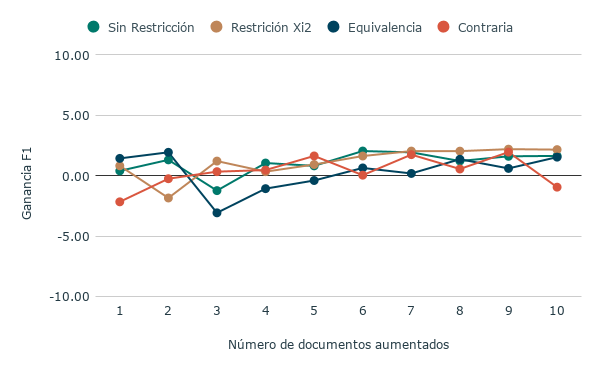
\includegraphics[width=\textwidth]{sections/figures/CNN_anox.png}
        \caption{CNN}
    \end{subfigure}

    
    \begin{subfigure}[b]{0.6\textwidth}
        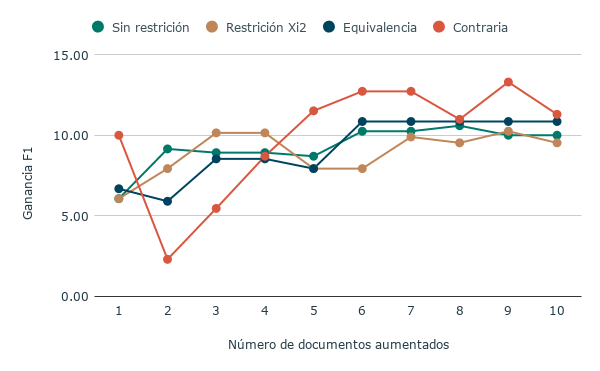
\includegraphics[width=\textwidth]{sections/figures/SVM-anorexia.png}
        \caption{SVM}
    \end{subfigure}
    
    \caption{Relación entre el número de documentos aumentados y la ganancia en F1 para el conjunto \textit{Anorexia}.}
    \label{fig:aumento_n_anorexia}
\end{figure}
\newpage

\subsection{Comparación con el estado del arte en detección de depresión y anorexia}
En las tablas \ref{table:dep1} y \ref{table:dep2} se comparan los resultados obtenidos mediante aumento de datos utilizando una red Bi-LSTM y aumento de datos, con los modelos evaluados en la conferencia eRISK 2018 \cite{Losada2018}. Para detección de depresión de un total de 45 modelos nuestra propuesta se puede ubicar en el quinto lugar. En la tabla \ref{table:dep2} de un total de 35 propuestas nuestro modelo quedaría en el segundo lugar. Es importante señalar que las propuestas ganadoras no utilizaron aumento de datos y la mayoría se enfocó a realizar extracción de características, por lo que dichas propuestas podrían mejorar mediante el aumento de datos propuesto.
\begin{table}[hbt!]
\caption{Resultados para el conjunto de depresión en términos de F1, en comparación con los modelos presentados en el eRISK 2018.} \label{table:dep1}
\begin{center}
    

\begin{tabular}{lccc}
\hline
{\color[HTML]{000000} \textbf{Modelo}}       & \multicolumn{1}{l}{{\color[HTML]{000000} \textbf{F1}}} & \multicolumn{1}{l}{{\color[HTML]{000000} \textbf{Precisión}}} & \multicolumn{1}{l}{{\color[HTML]{000000} \textbf{Recuerdo}}} \\ \hline
{\color[HTML]{000000} FHDO-BCSGB (Max)}      & {\color[HTML]{000000} 0.64}                            & {\color[HTML]{000000} 0.64}                                   & {\color[HTML]{000000} 0.65}                                  \\ \hline
{\color[HTML]{000000} \textbf{RNN+Aumento}}  & {\color[HTML]{000000} 0.56}                            & {\color[HTML]{000000} 0.57}                                   & \cellcolor[HTML]{F3FAF7}{\color[HTML]{000000} 0.54}          \\ \hline
{\color[HTML]{000000} Promedio (45 modelos)} & {\color[HTML]{000000} 0.42}                            & {\color[HTML]{000000} 0.37}                                   & {\color[HTML]{000000} 0.55}                                  \\ \hline
{\color[HTML]{000000} UDCE (Min)}            & {\color[HTML]{000000} 0.18}                            & {\color[HTML]{000000} 0.13}                                   & {\color[HTML]{000000} 0.29}                                  \\ \hline
\end{tabular}
\end{center}

\end{table}



\begin{table}[hbt!]
\caption{Resultados para el conjunto de anorexia en términos de F1, en comparación con los modelos presentados en el eRISK 2018.} \label{table:dep2}

\begin{center}

\begin{tabular}{lccc}
\hline
{\color[HTML]{000000} \textbf{Modelo}}       & \multicolumn{1}{l}{{\color[HTML]{000000} \textbf{F1}}} & \multicolumn{1}{l}{{\color[HTML]{000000} \textbf{Precision}}} & \multicolumn{1}{l}{{\color[HTML]{000000} \textbf{Recuerdo}}} \\ \hline
{\color[HTML]{000000} FHDO-BCSGE (Max)}      & {\color[HTML]{000000} 0.85}                            & {\color[HTML]{000000} 0.87}                                   & {\color[HTML]{000000} 0.83}                                  \\ \hline
{\color[HTML]{000000} \textbf{RNN+Aumento}}      & {\color[HTML]{000000} 0.83}                            & {\color[HTML]{000000} 0.84}                                   & \cellcolor[HTML]{F3FAF7}{\color[HTML]{000000} 0.81}          \\ \hline
{\color[HTML]{000000} Promedio (35 modelos)} & {\color[HTML]{000000} 0.56}                            & {\color[HTML]{000000} 0.63}                                   & {\color[HTML]{000000} 0.58}                                  \\ \hline
{\color[HTML]{000000} UNSLA (Min)}           & {\color[HTML]{000000} 0.17}                            & {\color[HTML]{000000} 0.57}                                   & {\color[HTML]{000000} 0.1}                                   \\ \hline
\end{tabular}

\end{center}


\end{table}
%Poner una tabla comparativa 


\subsection{Análisis del aumento de datos}
Con el objetivo de comprobar como afecta el aumento de datos a la originalidad y diversidad del documento original, se realizan dos tipos de análisis: estadísticas del aumento en el vocabulario y las palabras palabras más relevantes utilizadas para la restrición y ejemplos seleccionados.

\subsubsection{Aumento del vocabulario}
En la figura \ref{fig:aumento_vocab_dep} se representa la relación del número de palabras nuevas y el número de documentos aumentados, %para el conjunto de depresión 
se realiza la comparación de los diferentes métodos de aumento. Como se puede esperar conforme aumenta el número de documentos el vocabulario también lo hace. En las subfiguras (a) y (c) se compara el aumento del vocabulario para la clase positiva, en la cual el método basado en relaciones contrarias incrementa drásticamente el vocabulario desde un documento por cada instancia y el que menos agrega palabras es el basado en tesauro, debido a que el método tesauro utiliza el parámetro $p$ para selección igual a 0.5 por que en promedio solo remplaza 2 palabras por cada segmento a aumentar. Los métodos con y sin restricción agregan el mismo número de palabras debido a que solo difieren en que palabras reemplazar. Por otra parte el basado en relaciones de equivalencia agrega un mayor vocabulario a los dos anterior por lo que se logra el objetivo de insertar un vocabulario diferente al emplear un criterio de similitud diferente.

En la subfiguras \ref{fig:aumento_vocab_dep} (b) y (d), se compara el aumento del vocabulario considerando ambas clases, debido a que el aumento de datos propuesto se basa sobre la clase de interés (la clase positiva). Resalta el hecho de que aunque el método de equivalencias contrarias introduce un gran vocabulario en la clase positiva para el conjunto de depresión, solo agrega de 500 a 2000 mil palabras nuevas considerando ambas clases, sin embargo para el conjunto de anorexia agrega muchas más. Esto se debe al tamaño del conjunto dado que en el conjunto de anorexia existe un vocabulario menor en comparación con el de depresión.

%esto es debido a que se parte del vocabulario de la clase contraria (negativa) y se realizan pocas modificaciones para llevarla el segmento a la clase positiva.
En resumen el método que agrego mas vocabulario fue el basado en relaciones contrarias, seguido del basado en equivalencias. Es interesante que el método con restricción agrega la misma modificación que el que no la realiza y puede obtener mejores resultados, por lo que se comprueba la efectividad del metodo.

\begin{figure}[hbt!]
    \begin{subfigure}[b]{0.5\textwidth}
        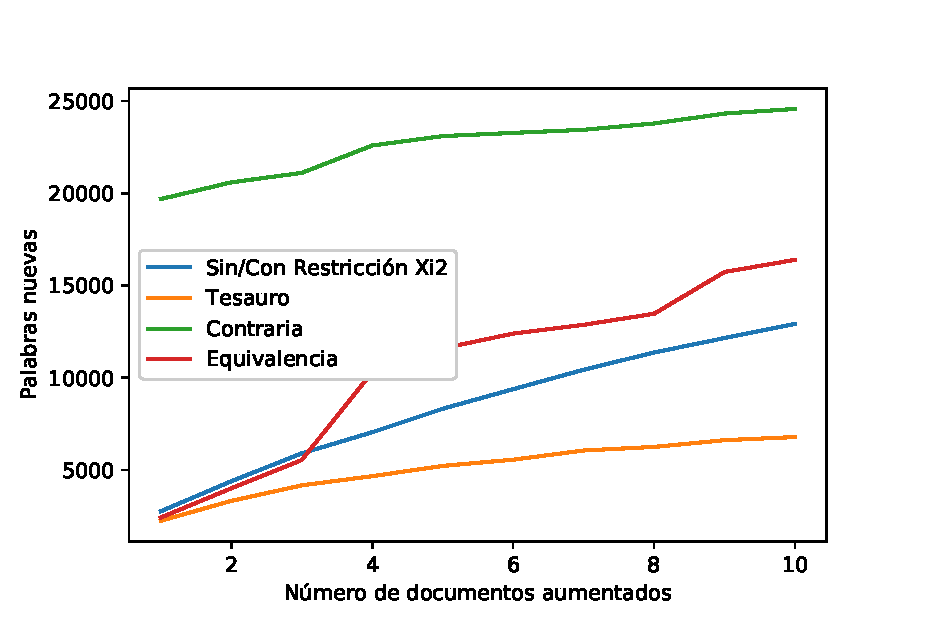
\includegraphics[width=\textwidth]{sections/figures/pos_plot.eps}
        \caption{Depresión: Clase positiva}
    \end{subfigure}
    \hfill
    \begin{subfigure}[b]{0.5\textwidth}
        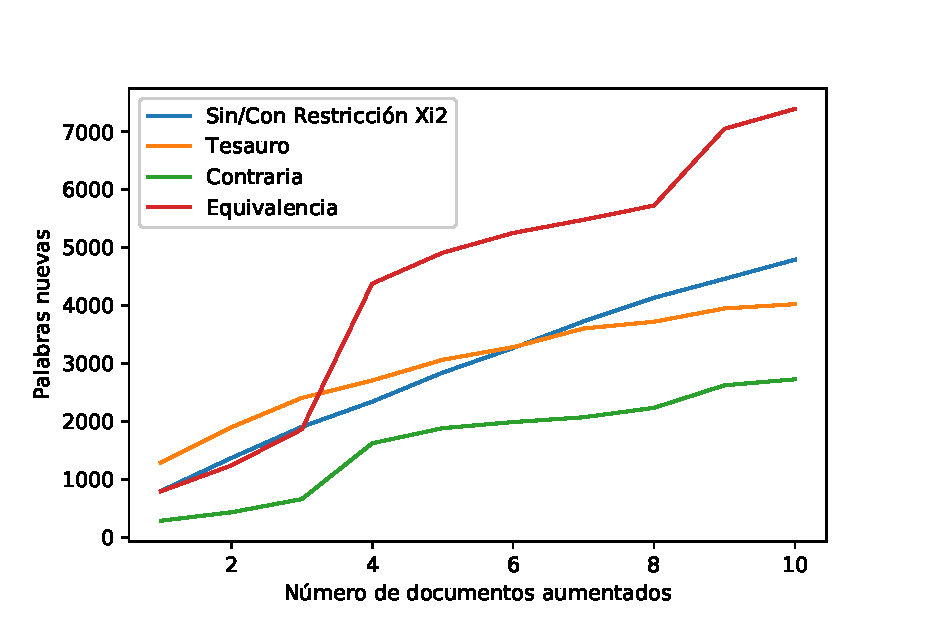
\includegraphics[width=\textwidth]{sections/figures/both_plot_1.eps}
        \caption{Depresion: Ambas clases}
    \end{subfigure}
    \hfill
    
    \begin{subfigure}[b]{0.5\textwidth}
        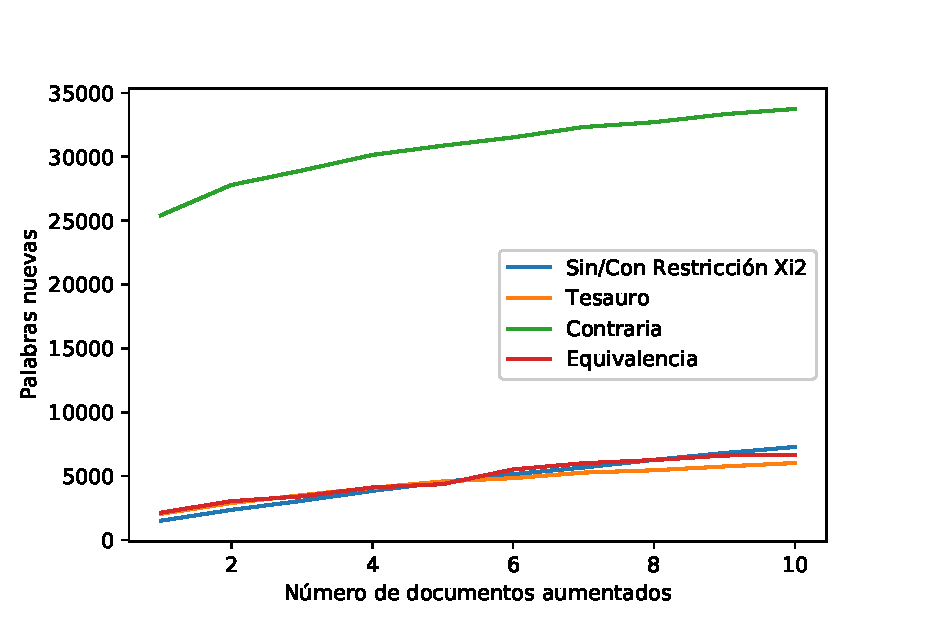
\includegraphics[width=\textwidth]{sections/figures/pos_plot_anox.eps}
        \caption{Anorexia: Clase positiva}
    \end{subfigure}
    \hfill
    \begin{subfigure}[b]{0.5\textwidth}
        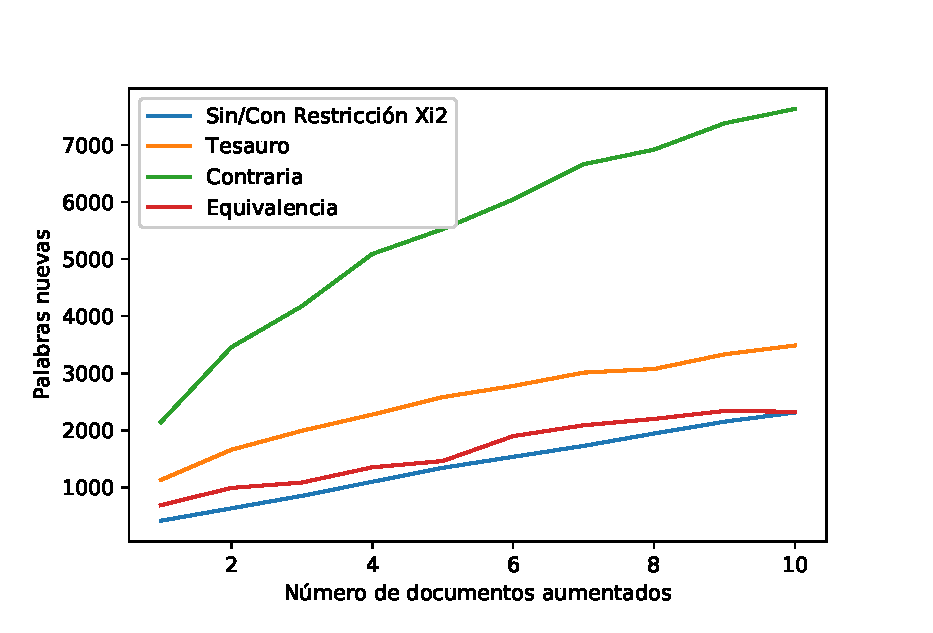
\includegraphics[width=\textwidth]{sections/figures/both_plot_anox.eps}
        \caption{Anorexia: Ambas clases}
    \end{subfigure}
    
    
    \caption{Relación entre el numero de documentos aumentados y el vocabulario nuevo agregado.}
    \label{fig:aumento_vocab_dep}
\end{figure}

\subsubsection{Palabras con mayor puntuación $\chi^2$}
En la figura \ref{fig:words_chi_anox}, se representan las palabras con mayor puntuación $\chi^2$ mismas que sirvieron para realizar el preprocesa miento y también para el método de aumento con restricción. La figura muestra las palabras mas importantes en un tamaño de fuente mas grande seguidas de las de menor importancia en una fuente mas pequeña. 

Como se ha demostrado en estudios previos las palabras relacionadas con pronombres personales y posesivos son mas utilizadas por personas con signos de depresión o anorexia, además de palabras relacionadas a relaciones personales como: ``boyfriend", ``feeling", ``friends", ``dating". Tambien sobre salen palabras relacionadas a la enfermedad como: ``meds", ``medication", ``anorexia", ``depression"; entre otras.

\begin{figure}[hbt!]
\centering
 \begin{subfigure}[b]{0.7\textwidth}
        \includegraphics[width=\textwidth]{sections/figures/chi2_words_anorexia.eps}
        \caption{Anorexia}
\end{subfigure}
\hfill
\hfill
 \begin{subfigure}[b]{0.7\textwidth}
        \includegraphics[width=\textwidth]{sections/figures/chi2_words_depresion.eps}
        \caption{Depresión}
\end{subfigure}
  
    \caption{Palabras con mayor puntuación $\chi^2$}
    \label{fig:words_chi_anox}
\end{figure}

\subsubsection{Ejemplos del aumento de datos}
En la tabla \ref{table:ejemplos_pos} se presentan diversos ejemplos de aumento, el método basado en tesauro agrega un vocabulario mas formal, en comparación con los basados en similitudes relacionales. El método basado en restricción $\chi^2$ conserva palabras importantes como ``feel", mientras que los otros no toman en consideración esto. Por otra parte el método basado en relaciones equivalentes agrega la palabra \textit{``unfortunate"} como una palabra relacionada a la palabra \textit{``unhappy"}.

La tabla \ref{table:ejemplos_contraria} presenta ejemplos del aumento basado en relaciones contrarias, las palabras relacionadas a un contexto feliz, son llevadas a un context contrario. Por ejemplo el vervo \textit{``talked"} es reemplazado por \textit{``complained"} y \textit{``bothered"}.
\begin{table}[hbt!]
\caption{Ejemplos del aumento de datos.} 
\label{table:ejemplos_pos}
\begin{center}

\begin{tabular}{ll}
\hline
\rowcolor[HTML]{EFEFEF} 
\textbf{Método} & \textbf{Secuencia}                                                            \\ \hline
\rowcolor[HTML]{FFFFFF} 
Sin Aumento     & a lot of the time i have trouble communicating why i feel so unhappy          \\ \hline
\rowcolor[HTML]{FFFFFF} 
Thesauro        & a lot of the time i hold trouble communicating why i feel thusly infelicitous \\ \hline
\rowcolor[HTML]{FFFFFF} 
Sin Restricción & a lots of the time i have trouble communicating why i feeling so unhappy      \\ \hline
\rowcolor[HTML]{FFFFFF} 
Restricción Xi2 & a lot of the time i have difficulty informing why i feel so unhappy           \\ \hline
\rowcolor[HTML]{FFFFFF} 
Equivalencia    & a much of the place i have troubles informing why i feeling so unfortunate    \\ \hline
\end{tabular}
\end{center}
\end{table}

\begin{table}[hbt!]
\caption{Ejemplos del aumento de datos para el método basado en relaciones opuestas.} 
\label{table:ejemplos_contraria}
\begin{center}

\begin{tabular}{ll}
\hline
\rowcolor[HTML]{EFEFEF} 
\textbf{Método} & \textbf{Secuencia}                                           \\ \hline
\rowcolor[HTML]{FFFFFF} 
Sin Aumento     & i connected with a girl we sat up and talked all night       \\ \hline
\rowcolor[HTML]{FFFFFF} 
Opuesta       & i disconnected with a girl we sat up and talked all night    \\ \hline
\rowcolor[HTML]{FFFFFF} 
Opuesta       & i connected with a girl we sat up and complained all night   \\ \hline
\rowcolor[HTML]{FFFFFF} 
Opuesta       & i connected with a boy we complained up and talked all night \\ \hline
\rowcolor[HTML]{FFFFFF} 
Opuesta       & i dispirited with a girl we sat up and talked all night      \\ \hline
\rowcolor[HTML]{FFFFFF} 
Opuesta       & i connected with a shy we dismayed up and bothered all night \\ \hline
\end{tabular}

\end{center}
\end{table}
%\subsection{Relación entre precisión y recuerdo}

%\subsection{Errores}

%\subsubsection{Tipo I: Falsos positivos}

%\subsubsection{Tipo II: Falsos negativos}